% Compile from the repository root:
% latexmk -pdf -outdir=output/pdf output/pdf/chapter-figure-design-review.tex
% REVIEW ONLY: neither this file nor the draft table is included by the chapter.
\documentclass[11pt,a4paper]{article}
\usepackage[margin=18mm,headheight=14pt]{geometry}
\usepackage[T1]{fontenc}
\usepackage{amsmath,amssymb,mathtools,bm,physics}
\usepackage{libertine}
\usepackage[libertine]{newtxmath}
\usepackage[table]{xcolor}
\usepackage{graphicx,booktabs,array,tabularx,microtype,fancyhdr}
\usepackage{tikz}
\usetikzlibrary{arrows.meta,positioning}
\usepackage{hyperref}
\graphicspath{{fig/}}
\definecolor{hfGreenDark}{HTML}{00574D}
\definecolor{hfGreen}{HTML}{00685C}
\definecolor{hfBlue}{HTML}{1769AA}
\definecolor{hfRed}{HTML}{B23A48}
\definecolor{hfOrange}{HTML}{D96C22}
\definecolor{hfViolet}{HTML}{775DA6}
\definecolor{hfPale}{HTML}{EDF2F6}
\definecolor{hfInk}{HTML}{202A33}
\hypersetup{colorlinks=true,urlcolor=hfGreen,linkcolor=hfGreen,
 pdftitle={HF chapter: proposed figure and table designs},
 pdfauthor={Pierre-Francois Loos}}
\pagestyle{fancy}
\fancyhf{}
\fancyhead[L]{\small\color{hfGreenDark}HF chapter: design review}
\fancyhead[R]{\small Draft -- not incorporated}
\fancyfoot[C]{\thepage}
\setlength{\parindent}{0pt}
\setlength{\parskip}{5pt}
\newcommand{\bS}{\boldsymbol S}
\newcommand{\bX}{\boldsymbol X}
\newcommand{\bU}{\boldsymbol U}
\newcommand{\bs}{\boldsymbol s}
\newcommand{\bR}{\boldsymbol R}
\newcommand{\br}{\boldsymbol r}
\newcommand{\chS}{\hat{\mathcal S}}
\newcommand{\chK}{\hat{\mathcal K}}
\newcommand{\heading}[2]{%
 {\LARGE\bfseries\color{hfGreenDark}#1\par}
 {\small\color{hfInk}#2\par}\vspace{2mm}}
\newcommand{\tagline}[1]{{\small\bfseries\color{hfGreenDark}#1\par}}
\newcommand{\credit}[1]{{\small\color{hfInk}#1\par}}
\newcommand{\nodeStyle}{}
\tikzset{
 nucleus/.style={circle,draw=hfGreenDark,fill=hfGreen!12,minimum size=7mm},
 electron/.style={circle,draw=hfBlue,fill=hfBlue!10,minimum size=7mm},
 old/.style={hfBlue,densely dashed,thick,-{Latex[length=2mm]}},
 new/.style={hfGreenDark,very thick,-{Latex[length=2mm]}},
 card/.style={draw=hfGreenDark,fill=hfGreen!5,rounded corners=2mm,
   align=center,minimum height=12mm},
 occupied/.style={circle,fill=hfGreenDark,inner sep=2.1pt},
 vacant/.style={circle,draw=hfInk!50,inner sep=2.1pt},
 hole/.style={circle,draw=hfRed,thick,inner sep=2.1pt},
 particle/.style={circle,fill=hfViolet,inner sep=2.1pt}}
\begin{document}

\heading{1. Molecular coordinates}{Proposed replacement for current Fig. 1}
\tagline{Current illustration}
\begin{center}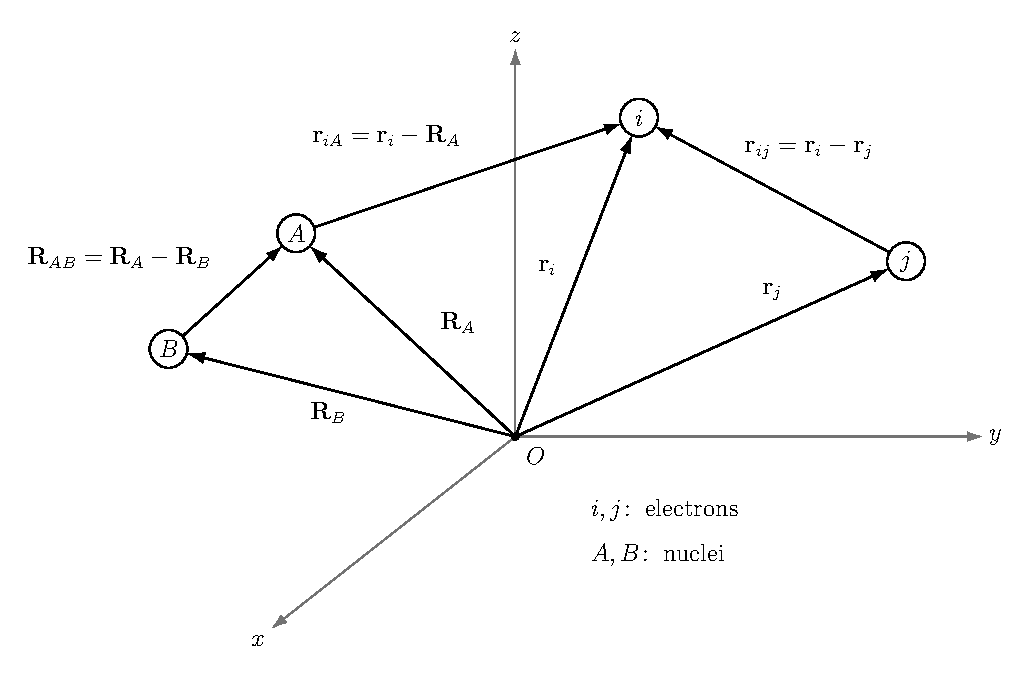
\includegraphics[height=43mm]{coord}\end{center}
\tagline{Proposed design: separate positions from displacements}
\begin{center}
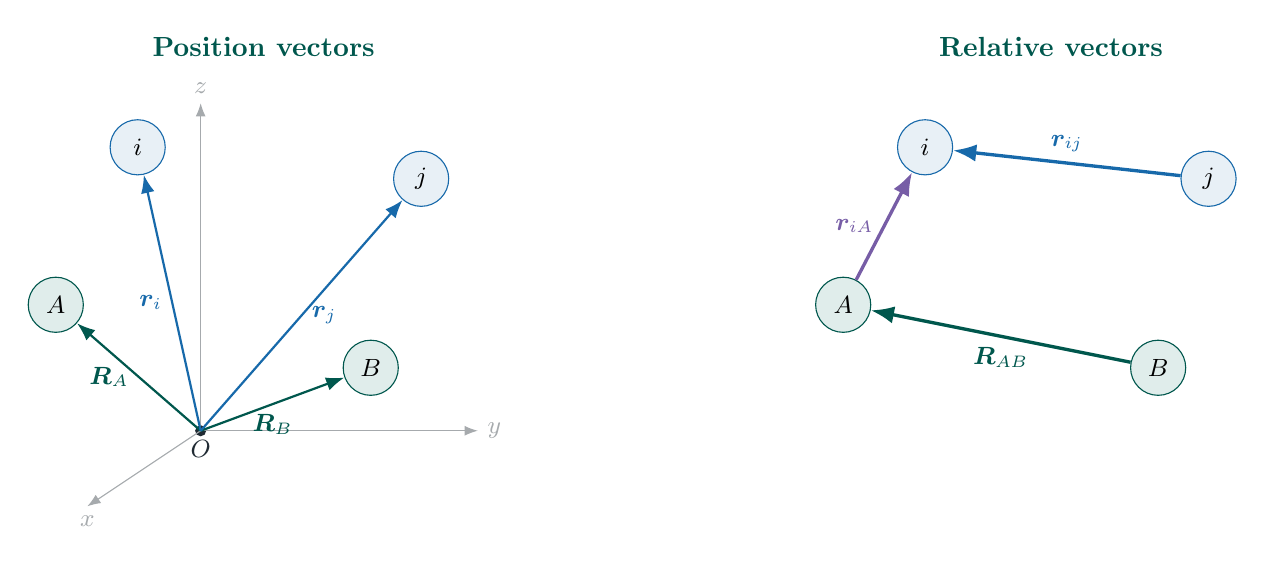
\begin{tikzpicture}[x=8mm,y=8mm,font=\small,>=Latex]
 \foreach \shift/\title in {0/Position vectors,10/Relative vectors}{
  \begin{scope}[xshift=\shift cm]
   \node[font=\bfseries,text=hfGreenDark] at (1,6.1) {\title};
   \coordinate (O) at (0,0);
   \node[nucleus] (A) at (-2.3,2.0) {$A$};
   \node[nucleus] (B) at (2.7,1.0) {$B$};
   \node[electron] (i) at (-1.0,4.5) {$i$};
   \node[electron] (j) at (3.5,4.0) {$j$};
   \ifnum\shift=0
    \fill[hfInk] (O) circle (2pt) node[below] {$O$};
    \draw[->,hfInk!40] (O)--(4.4,0) node[right] {$y$};
    \draw[->,hfInk!40] (O)--(0,5.2) node[above] {$z$};
    \draw[->,hfInk!40] (O)--(-1.8,-1.2) node[below] {$x$};
    \draw[->,hfGreenDark,thick] (O)--(A)
      node[midway,left] {$\bR_A$};
    \draw[->,hfGreenDark,thick] (O)--(B)
      node[midway,below] {$\bR_B$};
    \draw[->,hfBlue,thick] (O)--(i)
      node[midway,left] {$\br_i$};
    \draw[->,hfBlue,thick] (O)--(j)
      node[midway,right] {$\br_j$};
   \else
    \draw[->,hfViolet,very thick] (A)--(i)
      node[midway,left] {$\br_{iA}$};
    \draw[->,hfBlue,very thick] (j)--(i)
      node[midway,above] {$\br_{ij}$};
    \draw[->,hfGreenDark,very thick] (B)--(A)
      node[midway,below] {$\bR_{AB}$};
   \fi
  \end{scope}
 }
\end{tikzpicture}
\[
 \br_{iA}=\br_i-\bR_A\qquad
 \br_{ij}=\br_i-\br_j\qquad
 \bR_{AB}=\bR_A-\bR_B
\]
\end{center}
\credit{Nuclei: green; electrons: blue. The two panels use the same geometry.
New vector drawing following the coordinate definitions in Szabo and Ostlund,
\emph{Modern Quantum Chemistry}. The source credit will remain.}

\newpage
\heading{2. Restricted and unrestricted orbitals}{Proposed replacement for current Fig. 2}
\tagline{Current illustration}
\begin{center}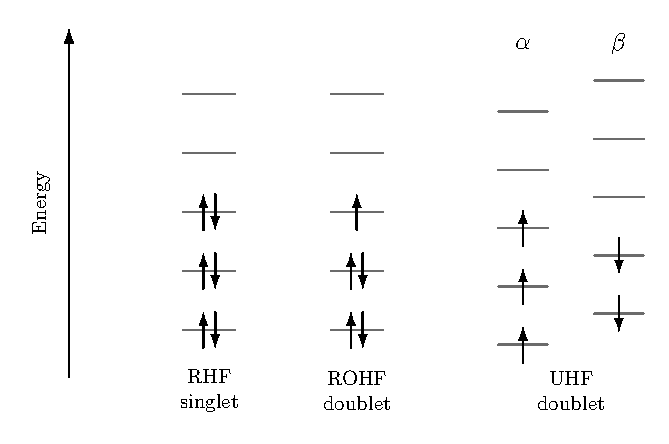
\includegraphics[height=47mm]{RHF_UHF}\end{center}
\tagline{Proposed design: show which spatial functions are shared}
\begin{center}
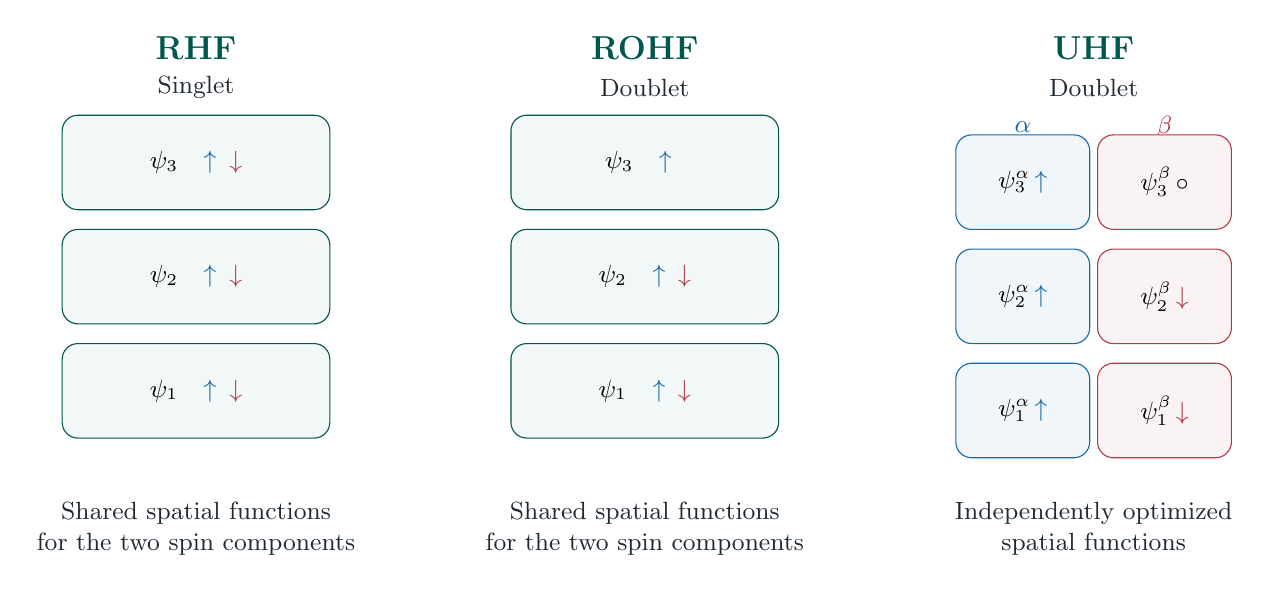
\begin{tikzpicture}[font=\small,x=1cm,y=1cm]
 \foreach \x/\title/\subtitle in {0/RHF/Singlet,5.7/ROHF/Doublet,11.4/UHF/Doublet}{
  \node[font=\large\bfseries,text=hfGreenDark] at (\x,0) {\title};
  \node[text=hfInk] at (\x,-0.5) {\subtitle};
 }
 \foreach \x in {0,5.7}{
  \foreach \r/\p in {1/3,2/2,3/1}{
   \node[card,minimum width=34mm] at (\x,-1.45*\r)
    {$\psi_{\p}$\quad
      \textcolor{hfBlue}{$\uparrow$}\,
      \ifnum\r=1\ifdim\x pt=0pt
      \textcolor{hfRed}{$\downarrow$}\fi
      \else\textcolor{hfRed}{$\downarrow$}\fi};
  }
  \node[align=center,text=hfInk] at (\x,-6.1)
   {Shared spatial functions\\for the two spin components};
 }
 \node[text=hfBlue] at (10.5,-1) {$\alpha$};
 \node[text=hfRed] at (12.3,-1) {$\beta$};
 \foreach \r/\p in {1/3,2/2,3/1}{
  \node[card,draw=hfBlue,fill=hfBlue!6,minimum width=17mm] at (10.5,-1.45*\r-0.25)
   {$\psi_{\p}^{\alpha}\,\textcolor{hfBlue}{\uparrow}$};
  \node[card,draw=hfRed,fill=hfRed!6,minimum width=17mm] at (12.3,-1.45*\r-0.25)
   {$\psi_{\p}^{\beta}\,\ifnum\r=1\circ\else\textcolor{hfRed}{\downarrow}\fi$};
 }
 \node[align=center,text=hfInk] at (11.4,-6.1)
   {Independently optimized\\spatial functions};
\end{tikzpicture}
\end{center}
\credit{Illustrative occupations retain the singlet/doublet examples and the
ROHF case in the source. This design emphasizes orbital sharing rather than
orbital-energy order; it is not an energy-level plot. New schematic following
Jensen, \emph{Introduction to Computational Chemistry}.}

\newpage
\heading{3. Determinant occupations}{Proposed coordinated designs for current Figs. 3, 4, and 5}
\tagline{Current occupation diagrams}
\begin{center}
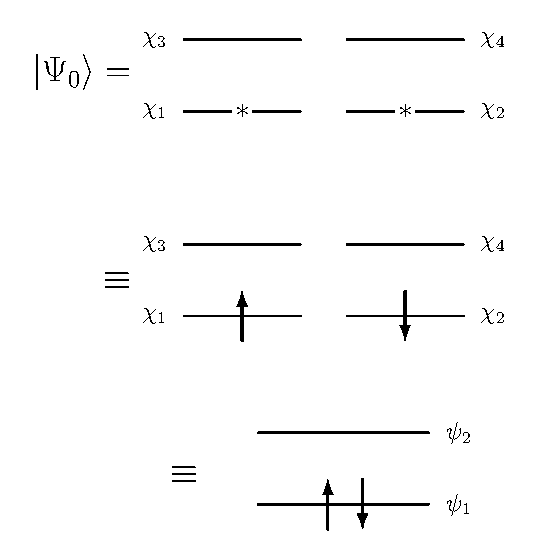
\includegraphics[height=33mm]{H2}\quad
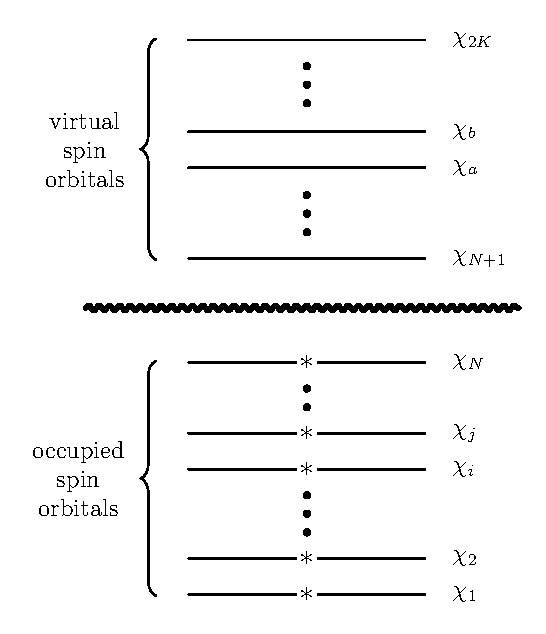
\includegraphics[height=33mm]{HF_det}\quad
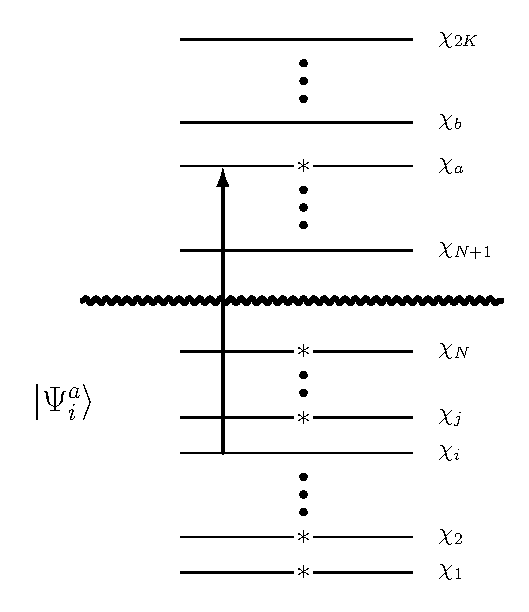
\includegraphics[height=33mm]{single}\quad
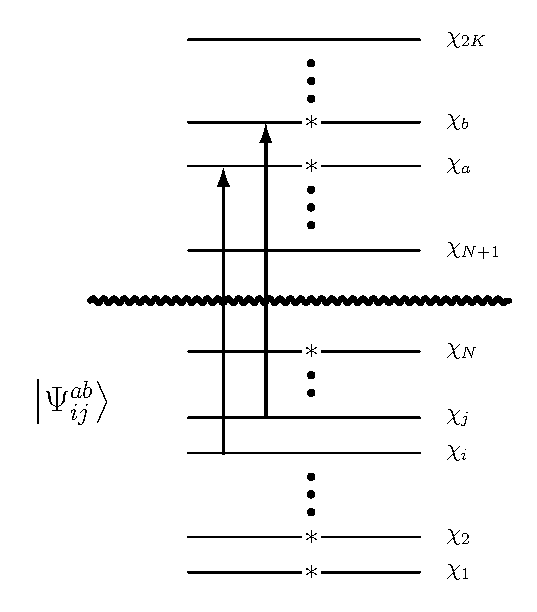
\includegraphics[height=33mm]{double}
\end{center}
\tagline{Proposed design: occupation maps in a common orbital basis}
\begin{center}
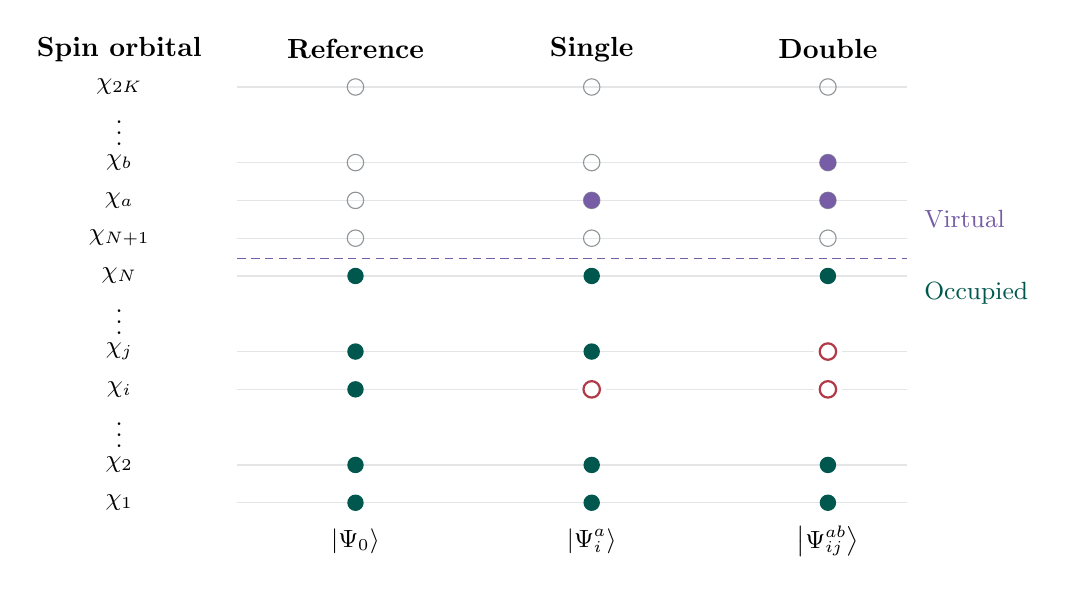
\begin{tikzpicture}[font=\small,x=1cm,y=1cm]
 \node[font=\bfseries] at (0,0) {Spin orbital};
 \node[font=\bfseries] at (3,0) {Reference};
 \node[font=\bfseries] at (6,0) {Single};
 \node[font=\bfseries] at (9,0) {Double};
 \foreach \r/\label in {1/{\chi_{2K}},2/{\vdots},3/{\chi_b},4/{\chi_a},
   5/{\chi_{N+1}},6/{\chi_N},7/{\vdots},8/{\chi_j},9/{\chi_i},
   10/{\vdots},11/{\chi_2},12/{\chi_1}}{
  \node at (0,-0.48*\r) {$\label$};
  \ifnum\r=2\else\ifnum\r=7\else\ifnum\r=10\else
   \draw[hfInk!12] (1.5,-0.48*\r)--(10,-0.48*\r);
   \foreach \x in {3,6,9}{
    \ifnum\r<6 \node[vacant] at (\x,-0.48*\r) {};
    \else \node[occupied] at (\x,-0.48*\r) {};\fi
   }
  \fi\fi\fi
 }
 \path[fill=white] (5.82,-4.48) rectangle (6.18,-4.17);
 \node[hole] at (6,-4.32) {};
 \node[particle] at (6,-1.92) {};
 \foreach \y in {-4.32,-3.84}{
  \path[fill=white] (8.82,\y-0.16) rectangle (9.18,\y+0.16);
  \node[hole] at (9,\y) {};
 }
 \node[particle] at (9,-1.92) {};
 \node[particle] at (9,-1.44) {};
 \draw[densely dashed,hfViolet] (1.5,-2.66)--(10,-2.66);
 \node[font=\small,text=hfViolet,anchor=west] at (10.1,-2.15) {Virtual};
 \node[font=\small,text=hfGreenDark,anchor=west] at (10.1,-3.1) {Occupied};
 \node at (3,-6.25) {$\ket{\Psi_0}$};
 \node at (6,-6.25) {$\ket{\Psi_i^a}$};
 \node at (9,-6.25) {$\ket{\Psi_{ij}^{ab}}$};
\end{tikzpicture}
\end{center}
\credit{Filled green: an unchanged occupied spin orbital; violet: a promoted
electron; red outline: a hole. Empty cells are unoccupied. Unshown occupations
remain unchanged. Rows show orbital labels, not numerical energies.}
\tagline{Closed-shell H$_2$: the same graphic vocabulary}
\[
 \underbrace{\chi_1=\alpha\psi_1,\quad\chi_2=\beta\psi_1}_{\text{occupied}}
 \qquad
 \underbrace{\chi_3=\alpha\psi_2,\quad\chi_4=\beta\psi_2}_{\text{virtual}}
 \qquad\Longleftrightarrow\qquad\psi_1^2
\]
\credit{New occupation-map layout following the determinant constructions of
Szabo and Ostlund, \emph{Modern Quantum Chemistry}. The source credit is retained.}

\newpage
\heading{4. Orthogonalization}{Proposed replacement for current Fig. 6}
\tagline{Current illustration}
\begin{center}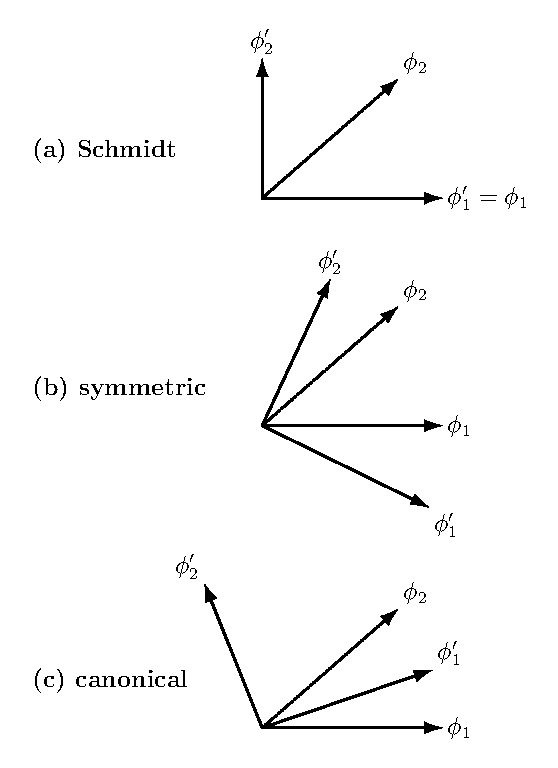
\includegraphics[height=47mm]{ortho}\end{center}
\tagline{Proposed design: parallel method panels and transformation rules}
\begin{center}
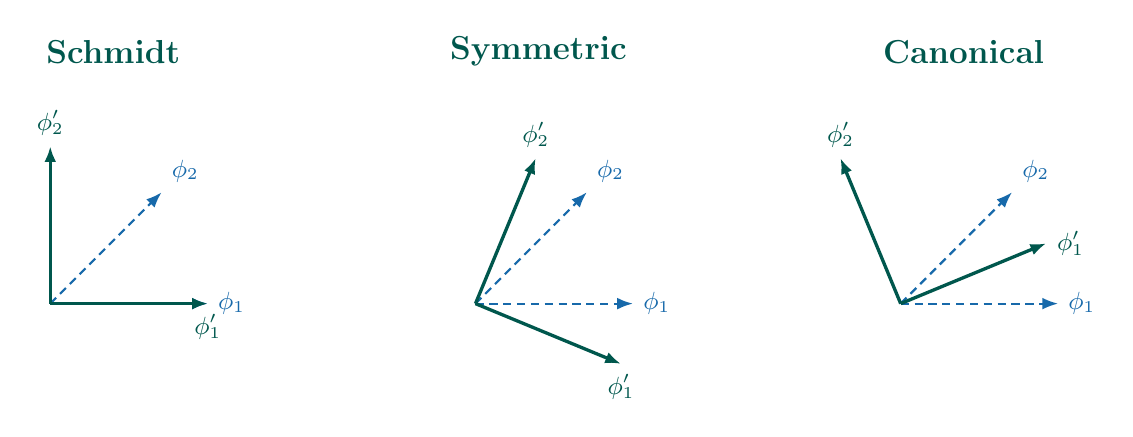
\begin{tikzpicture}[x=1cm,y=1cm,font=\small]
 \foreach \x/\method in {0/Schmidt,5.4/Symmetric,10.8/Canonical}{
  \begin{scope}[xshift=\x cm]
   \node[font=\large\bfseries,text=hfGreenDark] at (0.8,3.2) {\method};
   \draw[old] (0,0)--(2,0) node[right] {$\phi_1$};
   \draw[old] (0,0)--(1.414,1.414) node[above right] {$\phi_2$};
   \ifdim\x pt=0pt
    \draw[new] (0,0)--(2,0) node[below] {$\phi_1'$};
    \draw[new] (0,0)--(0,2) node[above] {$\phi_2'$};
   \else\ifdim\x pt=5.4pt
    \draw[new] (0,0)--(1.848,-0.765) node[below] {$\phi_1'$};
    \draw[new] (0,0)--(0.765,1.848) node[above] {$\phi_2'$};
   \else
    \draw[new] (0,0)--(1.848,0.765) node[right] {$\phi_1'$};
    \draw[new] (0,0)--(-0.765,1.848) node[above] {$\phi_2'$};
   \fi\fi
  \end{scope}
 }
\end{tikzpicture}
\vspace{4mm}
\begin{tabularx}{\linewidth}{>{\raggedright\arraybackslash}X
 >{\raggedright\arraybackslash}X >{\raggedright\arraybackslash}X}
\textcolor{hfGreenDark}{\textbf{Sequential}}&
\textcolor{hfGreenDark}{\textbf{Equal treatment}}&
\textcolor{hfGreenDark}{\textbf{Overlap eigenvectors}}\\[1mm]
Retain $\phi_1$; subtract its component from $\phi_2$ and normalize.&
$\bX=\bS^{-1/2}$&
$\bX=\bU\cdot\bs^{-1/2}$\\
\end{tabularx}
\[
 \bX^\dagger\cdot\bS\cdot\bX=\boldsymbol 1
\]
\end{center}
\credit{Dashed blue: original functions; solid green: orthonormal functions.
An illustrative pair of real normalized functions is used. Each green pair
is perpendicular; the methods choose different orthonormal coordinates in
the same space. Independently drawn panels following Szabo and Ostlund.}

\newpage
\heading{5. HF symmetry classes}{Proposed replacement for current Fig. 10}
\tagline{Current illustration}
\begin{center}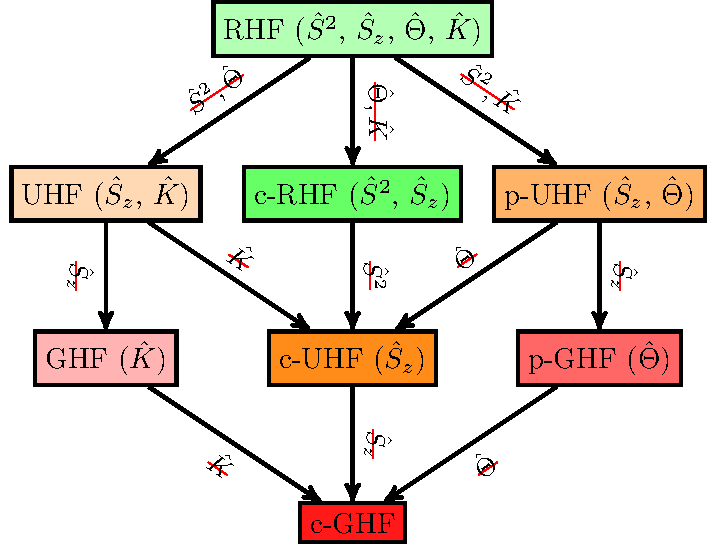
\includegraphics[height=47mm]{StuberPaldus}\end{center}
\tagline{Proposed design: constraint matrix plus explicit release map}
{\renewcommand{\arraystretch}{1.6}
\begin{tabularx}{\linewidth}{>{\bfseries}lXXX}
\toprule
Space & Real coefficients & Time-reversal paired & Complex coefficients\\
\midrule
\rowcolor{hfGreen!7}
RHF & RHF: $\chS^2,\chS_z,\chK,\hat\Theta$&
Not a separate class here&
c-RHF: $\chS^2,\chS_z$\\
\rowcolor{hfOrange!8}
UHF & UHF: $\chS_z,\chK$&
p-UHF: $\chS_z,\hat\Theta$&
c-UHF: $\chS_z$\\
\rowcolor{hfRed!6}
GHF & GHF: $\chK$&
p-GHF: $\hat\Theta$&
c-GHF: none of these\\
\bottomrule
\end{tabularx}}
\credit{Cells name the retained symmetries. Real and paired classes are
alternative constraints, not consecutive steps in an ordered chain.}
\tagline{All constraint-release connections retained from the original graph}
{\small\renewcommand{\arraystretch}{1.35}
\begin{tabularx}{\linewidth}{XX}
RHF $\to$ c-RHF: release $\hat\Theta,\chK$&
RHF $\to$ UHF: release $\chS^2,\hat\Theta$\\
RHF $\to$ p-UHF: release $\chS^2,\chK$&
c-RHF $\to$ c-UHF: release $\chS^2$\\
UHF $\to$ GHF: release $\chS_z$&
UHF $\to$ c-UHF: release $\chK$\\
p-UHF $\to$ p-GHF: release $\chS_z$&
p-UHF $\to$ c-UHF: release $\hat\Theta$\\
c-UHF $\to$ c-GHF: release $\chS_z$&
GHF $\to$ c-GHF: release $\chK$\\
p-GHF $\to$ c-GHF: release $\hat\Theta$&
\end{tabularx}}
\credit{New comparison layout based on Fig. 1 of Burton, Thom, and Loos,
\emph{Parity-Time Symmetry in Hartree-Fock Theory} (2019),
\href{https://doi.org/10.1021/acs.jctc.9b00289}{doi:10.1021/acs.jctc.9b00289}.
The chapter's existing Table 1 remains a separate, credited reproduction in
part from Henderson, Jimenez-Hoyos, and Scuseria (2018).}

\newpage
\heading{6. Carbon contraction data}{Proposed table replacing current Fig. 12}
\tagline{Current image excerpt}
\begin{center}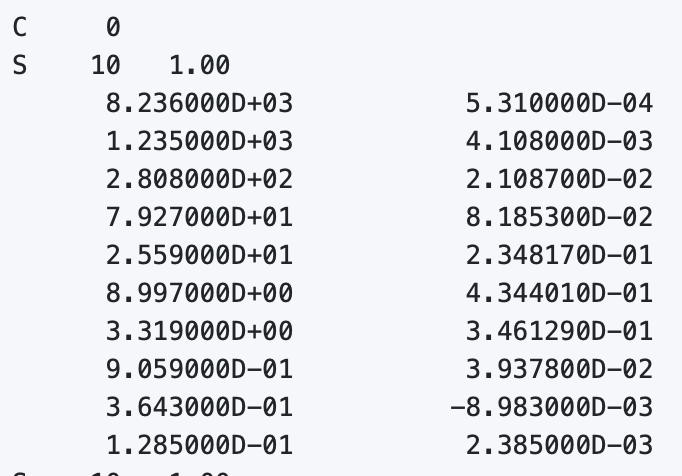
\includegraphics[height=48mm]{C}\end{center}
\tagline{Proposed native LaTeX table}
\begin{center}
{\renewcommand{\arraystretch}{1.22}
% Draft replacement for the current Figure 12. Not included in the chapter.
% Values transcribed from fig/C.png and checked against Basis Set Exchange.
% Scientific notation preserves every digit in the source excerpt.
\begin{tabular}{crr}
\toprule
Primitive $i$ & Exponent $\alpha_i$ & Coefficient $D_i$\\
\midrule
1  & $8.236000\times10^{3}$  & $5.310000\times10^{-4}$\\
2  & $1.235000\times10^{3}$  & $4.108000\times10^{-3}$\\
3  & $2.808000\times10^{2}$  & $2.108700\times10^{-2}$\\
4  & $7.927000\times10^{1}$  & $8.185300\times10^{-2}$\\
5  & $2.559000\times10^{1}$  & $2.348170\times10^{-1}$\\
6  & $8.997000\times10^{0}$  & $4.344010\times10^{-1}$\\
7  & $3.319000\times10^{0}$  & $3.461290\times10^{-1}$\\
8  & $9.059000\times10^{-1}$ & $3.937800\times10^{-2}$\\
9  & $3.643000\times10^{-1}$ & $-8.983000\times10^{-3}$\\
10 & $1.285000\times10^{-1}$ & $2.385000\times10^{-3}$\\
\bottomrule
\end{tabular}
}
\end{center}
\credit{\textbf{Proposed caption.} Primitive exponents and coefficients of
one ten-primitive $s$ contraction for carbon in cc-pVTZ. Shell scale: 1.00.
Values transcribed from the lecture excerpt and checked against the
\href{https://www.basissetexchange.org}{Basis Set Exchange}; basis family:
Dunning (1989), \href{https://doi.org/10.1063/1.456153}{doi:10.1063/1.456153}.}
\credit{Only the complete ten-row contraction visible in the image is included.
Every exponent and coefficient, including the negative ninth coefficient,
is retained exactly. The raw D-format notation is replaced by standard
scientific notation; the values have not been rounded or renormalized.}
\vspace{3mm}
\fcolorbox{hfGreenDark}{hfGreen!5}{\parbox{0.94\linewidth}{%
\textbf{Approval pending.} The chapter still contains the original Fig. 12.
This table and all proposed redraws are separate review material.
No replacement will be incorporated until you approve it.}}
\end{document}
